\documentclass[11pt]{article}
\usepackage{fullpage}
\usepackage{graphicx}
\usepackage{hyperref}
\begin{document}

\title{Homework 3 -- Precomputed Radiance Transfer}
\author{Gabe Fierro and Graham Tremper}
\date{\today}
\maketitle

\section{Introduction}

\section{Basic Relighting}

For the basic relighting viewer, we start by computing the light transport
matrix using cubemap pixel lights. A separate transport matrix is used for each
color channel. We raytrace the columns of the matrix using the open source
POVray ray-tracer with each column representing the scene lit from a single
cubemap pixel. This allows us to re-create an arbitrarily lit scene by linearly
combining the rows of the transport matrix with the weight of the light at the
corresponding cubemap pixel. We can do this in real-time without compression if
a limited number of cubemap lights are used.

\begin{table}[htb]
    \centering
    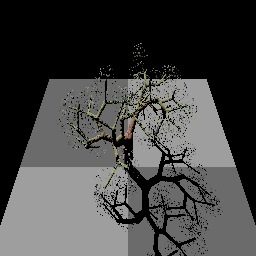
\includegraphics[width=.2\linewidth]{figs/tree/0000}
    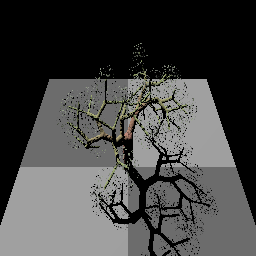
\includegraphics[width=.2\linewidth]{figs/tree/0001}
    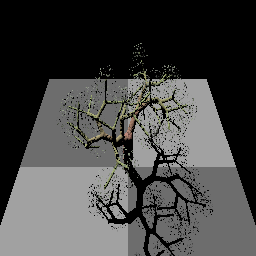
\includegraphics[width=.2\linewidth]{figs/tree/0002}
    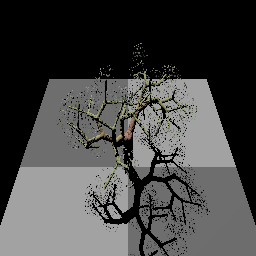
\includegraphics[width=.2\linewidth]{figs/tree/0003}
    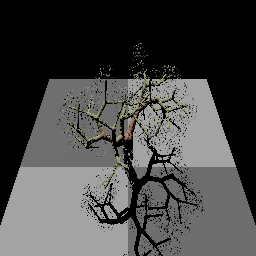
\includegraphics[width=.2\linewidth]{figs/tree/0004}
    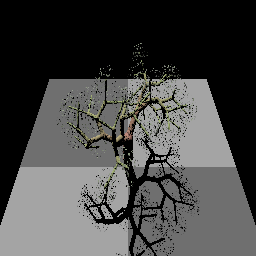
\includegraphics[width=.2\linewidth]{figs/tree/0005}
    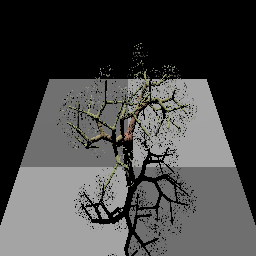
\includegraphics[width=.2\linewidth]{figs/tree/0006}
    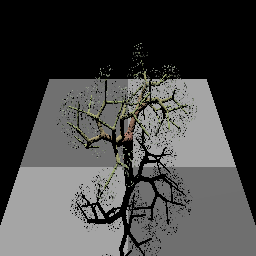
\includegraphics[width=.2\linewidth]{figs/tree/0007}
    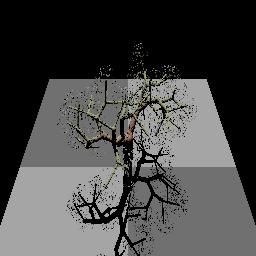
\includegraphics[width=.2\linewidth]{figs/tree/0008}
    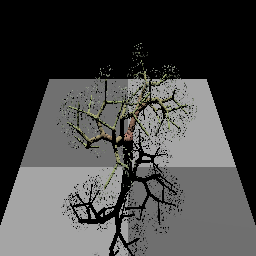
\includegraphics[width=.2\linewidth]{figs/tree/0009}
    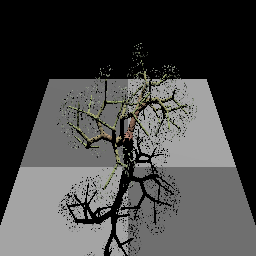
\includegraphics[width=.2\linewidth]{figs/tree/0010}
    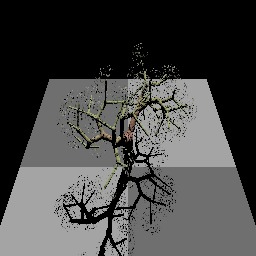
\includegraphics[width=.2\linewidth]{figs/tree/0011}
    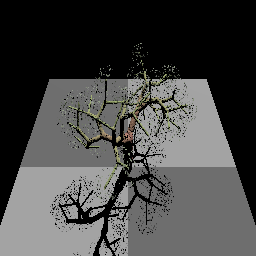
\includegraphics[width=.2\linewidth]{figs/tree/0012}
    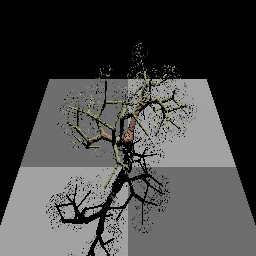
\includegraphics[width=.2\linewidth]{figs/tree/0013}
    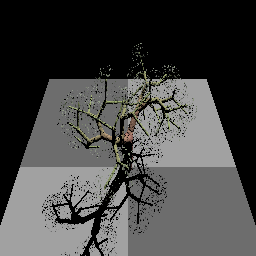
\includegraphics[width=.2\linewidth]{figs/tree/0014}
    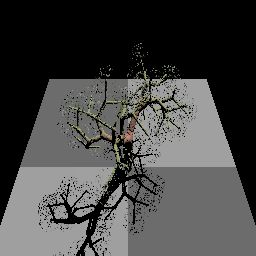
\includegraphics[width=.2\linewidth]{figs/tree/0015}
    \caption{16 of the 256 images generated by sweeping a light across the back of the bounding cube}
\end{table}

\subsection{Using POVray}

While POVray (http://povray.org/) is a fully-featured raytracer, it has several
limitations that made it difficult to efficiently and easily generate the large
number of images needed to compute the light transport matrix. Firstly, POVray
is single threaded, so generating all 6144 images for $32\times 32$ pixel
environment map (for all 6 sides of the cube), rendering the scene at
$512\times 512$ pixels at 3 seconds per render, takes over 5 hours, generating
over 1.3 GB of data.

\begin{center}
\begin{tabular}{|l|c|}
 \hline
 E.V. Dimension & Total Images\\
 \hline
 $4\times 4$ & 96 \\
 $16\times 16$ & 1536 \\
 $32\times 32$ & 6144 \\
 \hline
\end{tabular}
\end{center}

Secondly, POVray's default settings for rendering scenes make it difficult to
automate generating the images with the necessary contrast from each side of
the bounding cube. While POVray does contain a Turing-complete scripting
language, it only provides a single counter variable for generating successive
scenes, complicating the 2-dimensional parameterization of each face of the
cube.

\section{Environment Maps}

Once we light transport matrix is computing, adding an environment map is
straightforward. We used environments from ``Paul Debevec's'' website,
including Grace Cathedral, a eucalyptus grove, and a beach scene. Rendering the
scene simply involves weighting each column of the transport matrix by the
intensity of the corresponding pixel on the cubemap. Without compression,
real-time frame rate become intractable with large environment maps and output
image resolutions.

\begin{table}[htb]
    \centering
    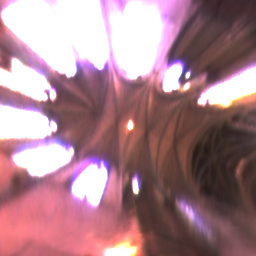
\includegraphics[width=.1\linewidth]{figs/grace/Grace0}
    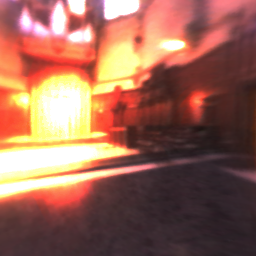
\includegraphics[width=.1\linewidth]{figs/grace/Grace1}
    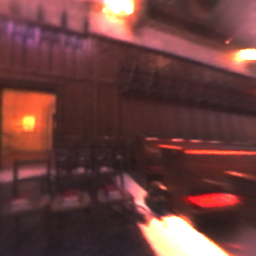
\includegraphics[width=.1\linewidth]{figs/grace/Grace2}
    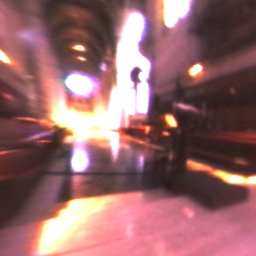
\includegraphics[width=.1\linewidth]{figs/grace/Grace3}
    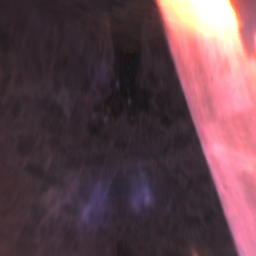
\includegraphics[width=.1\linewidth]{figs/grace/Grace4}
    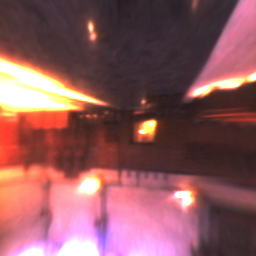
\includegraphics[width=.1\linewidth]{figs/grace/Grace5}
    \caption{Grace Cathedral environment map projected onto 6 sides of a bounding cube}
\end{table}

\section{Wavelet Transform}

In order to allow for larger scenes with higher resolution environment maps, we
used a Haar wavelet transform along each row of the light transport matrix.
Since each of these rows is essentially an environment map, we did a 2d Haar
transform for each face of the ``cube''. When rendering a frame, we haar
transform the current orientation of environment and then perform a sparse
matrix multiplication, using only the most significant terms. Ng et al. 03
suggested three methods of selecting subset of wavelet basis lights. These are
a naive ``unweighted selection'' which only looks at the wavelet coefficients and
a``transport-weighted selection'' which wights each wavelet coefficient by the
energy in the $i^{th}$ column of the transport matrix.

\begin{table}
  \centering
  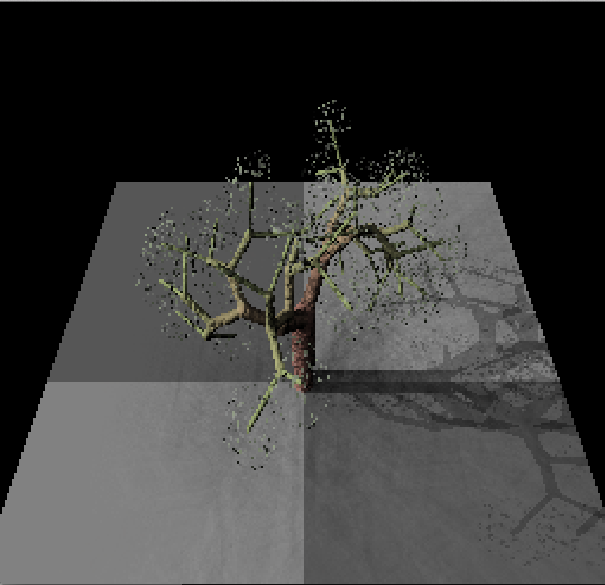
\includegraphics[width=.4\linewidth]{figs/naive}
  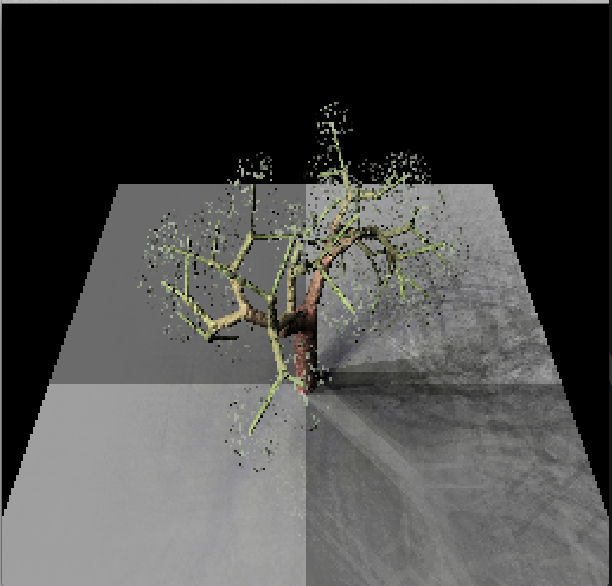
\includegraphics[width=.4\linewidth]{figs/weighted}
  \caption{Naive selection (left) vs Weighted selecting (right)}
\end{table}



\end{document}
